We begin this thesis by examining unitary matrices and their fundamental properties.
Next, we introduce the Cayley transform to finally approach the concept of spectral density.
Upon this we will be well-equipped to proceed with the investigation afterwards.

\section{Unitary Matrices}

We first recall two definitions for important real matrices that we then extend to complex matrices.
The index $^T$ marks the transpose of a matrix.
As common in literature, $I_n$ denotes the identity matrix of size $n$.

\begin{definition}[Symmetric matrix]
    Let $A$ be a real, square matrix of size $n$.
    Then $A$ is called \emph{symmetric} if $A^T = A$.
\end{definition}

The following definition is for matrices with their transpose as their inverse.

\begin{definition}[Orthogonal matrix]
    Let $A$ be a real, square matrix of size $n$.
    Then $A$ is called \emph{orthogonal} if $A^T \cdot A = A \cdot A^T = I_n$.
\end{definition}


Now we define the complex equivalent of a real symmetric matrix.
Here, $A^*$ denotes the \emph{conjugate transpose} (also called adjoint) of $A$, that is,
the matrix obtained by taking the transpose and then complex conjugating all entries.

\begin{definition}[Hermitian matrix]
    Let $A$ be a complex square matrix of size $n$.
    Then $A$ is called \emph{Hermitian} if $A^* = A$.
\end{definition}

Throughout this thesis, $A$ will denote a complex, square matrix of size $n$, unless stated otherwise.
When referring to a Hermitian matrix, we will use the letter $H$.

We now examine the eigenvalues of Hermitian matrices.

Let $H = H^*$ and $H v = \lambda v$ for a complex vector $v \neq \mathbf{0}$ of size $n$ and a scalar $\lambda \in \C$.
Consider now the inner product $ v^* v$.
Remember that $(A \cdot B)^* = B^* \cdot A^*$ holds for a matrix product,
and obviously ${(A^*)^*} = A$ for all matrices and vectors.

\[
    \lambda v^* v = v^* \left( \lambda v \right)
    = v^* \left( H v \right)
    = \left(v^* H \right) v
    = \left( H^* v \right)^* v
    = \left( H v \right)^* v
    = (\lambda v)^* v
    = \overline{\lambda} v^* v
\]

Since we have that $v \neq \mathbf{0}$ it follows that $v^* v \neq \mathbf{0}$
and therefore $\lambda = \overline{\lambda}$, that is to say $\lambda$ is real.
This means that all eigenvalues of Hermitian matrices are real numbers.
It follows that all eigenvalues of symmetric matrices are also real numbers,
since they are a special case of Hermitian matrices.
Now we can define the complex equivalent of orthogonal matrices:

\begin{definition}[Unitary matrix]
    A matrix $A$ is called \emph{unitary} if $A^* \cdot A = A \cdot A^* = I_n$.
\end{definition}

We will oftentimes denote unitary matrices by using $U$ as a reference.
It is easy to see that orthogonal matrices are a special case of unitary matrices,
since $A^T = A^*$ for all real matrices.\\
Consider a unitary matrix $U$ and an eigenpair $(\lambda, v)$ of $U$.
The complex conjugate of the eigenvalue equation $U v = \lambda v$ is

\[
    v^* U^* = v^* \overline{\lambda} = \overline{\lambda} v^*
\]

We calculate

\[
    v^* v = v^* I_n v = v^* U^* U v = v^* \overline{\lambda} \lambda v = \overline{\lambda} \lambda v^* v = \left| \lambda \right|^2 v^* v
\]

Similarly to above, we can divide by $v^* v$ to obtain

\[
    1 = \left| \lambda \right|^2 \implies \left| \lambda \right| = 1
\]

meaning that all eigenvalues of unitary matrices have a length of $1$ and are thus situated on the unit circle.
As they are a special case of unitary matrices, the same goes for orthogonal matrices.
This property is crucial, as it enables the application of the Cayley transform,
introduced in the following section.

There is a special group of matrices that all the matrices we have defined so far belong to.

\begin{definition}[Normal matrix]
    A matrix $A$ is called \emph{normal} if it commutes with its conjugate transpose,
    that is to say $A^* A = A A^*$.
\end{definition}

It is straightforward to see that both Hermitian and unitary matrices are normal matrices
and that the notion includes real symmetric and orthogonal matrices as special cases.\\
The spectral theorem states that normal matrices can be diagonalized by a unitary matrix.
That means, for any normal matrix $A$, there exists a unitary matrix $U$ such that $A = U \Lambda U^*$,
where $\Lambda = \diag(\lambda_1, \ldots, \lambda_n)$ with $\lambda_1, \ldots, \lambda_n$ being the eigenvalues of $A$.
This is essential for applying a function to a matrix, which we will get to in the next section.

\section{Cayley Transform}

Before giving the central definition of this section,
we will first extend the concept of functions to normal matrices,
allowing us to map one matrix to another.

\begin{definition}[Matrix function on normal matrices]
    Let $A$ be a normal matrix and let $f: \C \to \C$ be a function that is defined on the spectrum of $A$,
    $\sigma(A) = \{\lambda_1, \ldots, \lambda_n\}$.
    Then the \emph{matrix function} $f(A)$ is defined as
    \[
    f(A) := U f(\Lambda) U^* = U \diag(f(\lambda_1), \ldots, f(\lambda_n)) U^*
    \]
    where $U$ is the matrix of eigenvectors of $A$ and $\Lambda = \diag(\lambda_1, \ldots, \lambda_n)$ is the diagonal matrix of eigenvalues.
\end{definition}

Now we can define the \emph{Cayley transform}, which is a specific matrix function, 
that establishes a correspondence between Hermitian and unitary matrices,
allowing spectral properties to be translated between these two important classes.

For a complex number $z \in \mathbb{C}$ with $z \neq -i$, the Cayley transform is defined as
\[
\varphi(z) = \frac{i - z}{i + z}.
\]

This function maps the real line to the unit circle in the complex plane.

\vspace{0.5cm}

\begin{figure}[ht]
    \centering
    \begin{tikzpicture}

        % The real line
        \begin{axis}[
            axis lines = middle,
            name = realline,
            height = 4cm, width = 4cm,
            major tick length = 2ex,
            scale only axis,
            xlabel={$\re$},
            xlabel style = {
                at={(1.075,0.435)},
                anchor=south
            },
            ylabel={$\im$},
            ylabel style = {
                at={(0.415,1.07)},
                anchor=west
            },
            xmin = -2.5, xmax = 2.5,
            xtick = {-2,-1,1,2},
            ymin = -1.5, ymax = 1.5,
            ytick = {-1,1},
            yticklabels={$-i$,$i$}
        ]

            % (-\inf, -1)
            \addplot[
                domain = -3:-1,
                color = orange,
                style = thick
            ]
            ({x},{0});

            % [-1, 1]
            \addplot[
                domain = -1:1,
                color = blue,
                style = thick
            ]
            ({x},{0});

            % (1, \inf)
            \addplot[
                domain = 1:2.4,
                color = red,
                style = thick
            ]
            ({x},{0});

        \end{axis}

        % Cayley Transform
        \begin{axis}[
            at={(realline.east)},
            xshift=2.5cm,
            anchor=west,
            axis lines = middle,
            name = cayleytransform,
            height = 4cm, width = 4cm,
            scale only axis,
            xlabel={$\re$},
            xlabel style = {
                at={(1.075,0.435)},
                anchor=south
            },
            ylabel={$\im$},
            ylabel style = {
                at={(0.415,1.07)},
                anchor=west
            },
            ticks=none,
            xmin = -1.5, xmax = 1.5,
            ymin = -1.5, ymax = 1.5
        ]
            
            % Unit circle
            \addplot[
                domain = 0 : 2*pi,
                samples = 100
            ]
            ({cos(deg(x))}, {sin(deg(x))});

            % Image of (-\inf, -1)
            \addplot[
                domain = -200 : -1,
                color = orange,
                style = thick,
                samples = 1150
            ]
            ({(1 - x*x)/(1 + x*x)}, {(2*x)/(1 + x*x)});

            % Image of [-1, 1]
            \addplot[
                domain = -1 : 1,
                color = blue,
                style = thick,
                samples = 100
            ]
            ({(1 - x*x)/(1 + x*x)}, {(2*x)/(1 + x*x)});

            % Image of (1, \inf)
            \addplot[
                domain = 1 : 200,
                color = red,
                style = thick,
                samples = 1150
            ]
            ({(1 - x*x)/(1 + x*x)}, {(2*x)/(1 + x*x)});

        \end{axis}

        \path[->,out=45,in=135] 
            ($(realline.east)+(-0.5cm,1cm)$) edge
            node[auto,above] {$\varphi(z)$}
            ($(cayleytransform.west)+(0.5cm,1cm)$);

    \end{tikzpicture}
\end{figure}

% The real and imaginary values for the plots are calculated as follows:
%
%
% i - x    (i - x) * (i - x)     -1 - 2ix + x*x     -1 + x*x         -2x        1 - x*x         2x
% ----- = ------------------- = ---------------- = ---------- + i ---------- = --------- + i ---------
% i + x    (i + x) * (i - x)        -1 - x*x        -1 - x*x       -1 - x*x     1 + x*x       1 + x*x

For matrices, the Cayley transform maps a Hermitian matrix $H$ (with $i + H$ invertible) to a unitary matrix $U$ via
\[
U = (i - H)(i + H)^{-1}.
\]
The condition of $i + H$ being invertible is the same as requiring that $H$ does not have $-i$ as an eigenvalue.
If (and only if) that were the case, then we had $H v = -i v$ for some eigenvector $v \neq \mathbf{0}$,
and therefore 
\[
(i + H) v = i v + H v = i v + (-i v) = 0.
\]

Since Hermitian matrices have only real eigenvalues as discussed above, $-i$ can never be an eigenvalue.
Conversely, given a unitary matrix $U$ (with $U \neq -I_n$),
the inverse Cayley transform yields a Hermitian matrix:
\[
H = i (I_n - U)(I_n + U)^{-1}.
\]

This will be relevant later, as we can then use $\varphi$ to transform unitary matrices into symmetric ones and vice versa.

\subsection*{On the Choice of Random Unitary Matrices}


When generating random unitary matrices for numerical experiments,
it is important to ensure that their eigenvalues are distributed uniformly on the unit circle,
as predicted by random matrix theory.
A common approach is to generate a random complex matrix $A$ with independent standard normal entries
and then construct a unitary matrix from $A$ using either the QR decomposition or the singular value decomposition (SVD).
In the QR approach, $A$ is factored as $A = QR$, where $Q$ is unitary and $R$ is upper triangular.
The matrix $Q$ is then used as the random unitary matrix.
In the SVD approach, $A$ is factored as $A = U \Sigma V^*$,
and either $U$ or $V$ (both unitary) can be used as a random unitary matrix.
Although both methods produce unitary matrices, their statistical properties differ.
The SVD-based approach yields unitary matrices whose eigenvalues are uniformly distributed on the unit circle,
matching the theoretical prediction for random unitary matrices (the so-called Haar measure).
In contrast, the QR-based approach does not generally produce a uniform distribution of eigenvalues on the unit circle.
This distinction is important for applications where the spectral properties of random unitary matrices play a central role,
such as in the study of spectral densities.
For such purposes, the SVD-based construction is preferable,
as it ensures the correct statistical behavior of the eigenvalues.

\begin{figure}[htb]
    \centering
    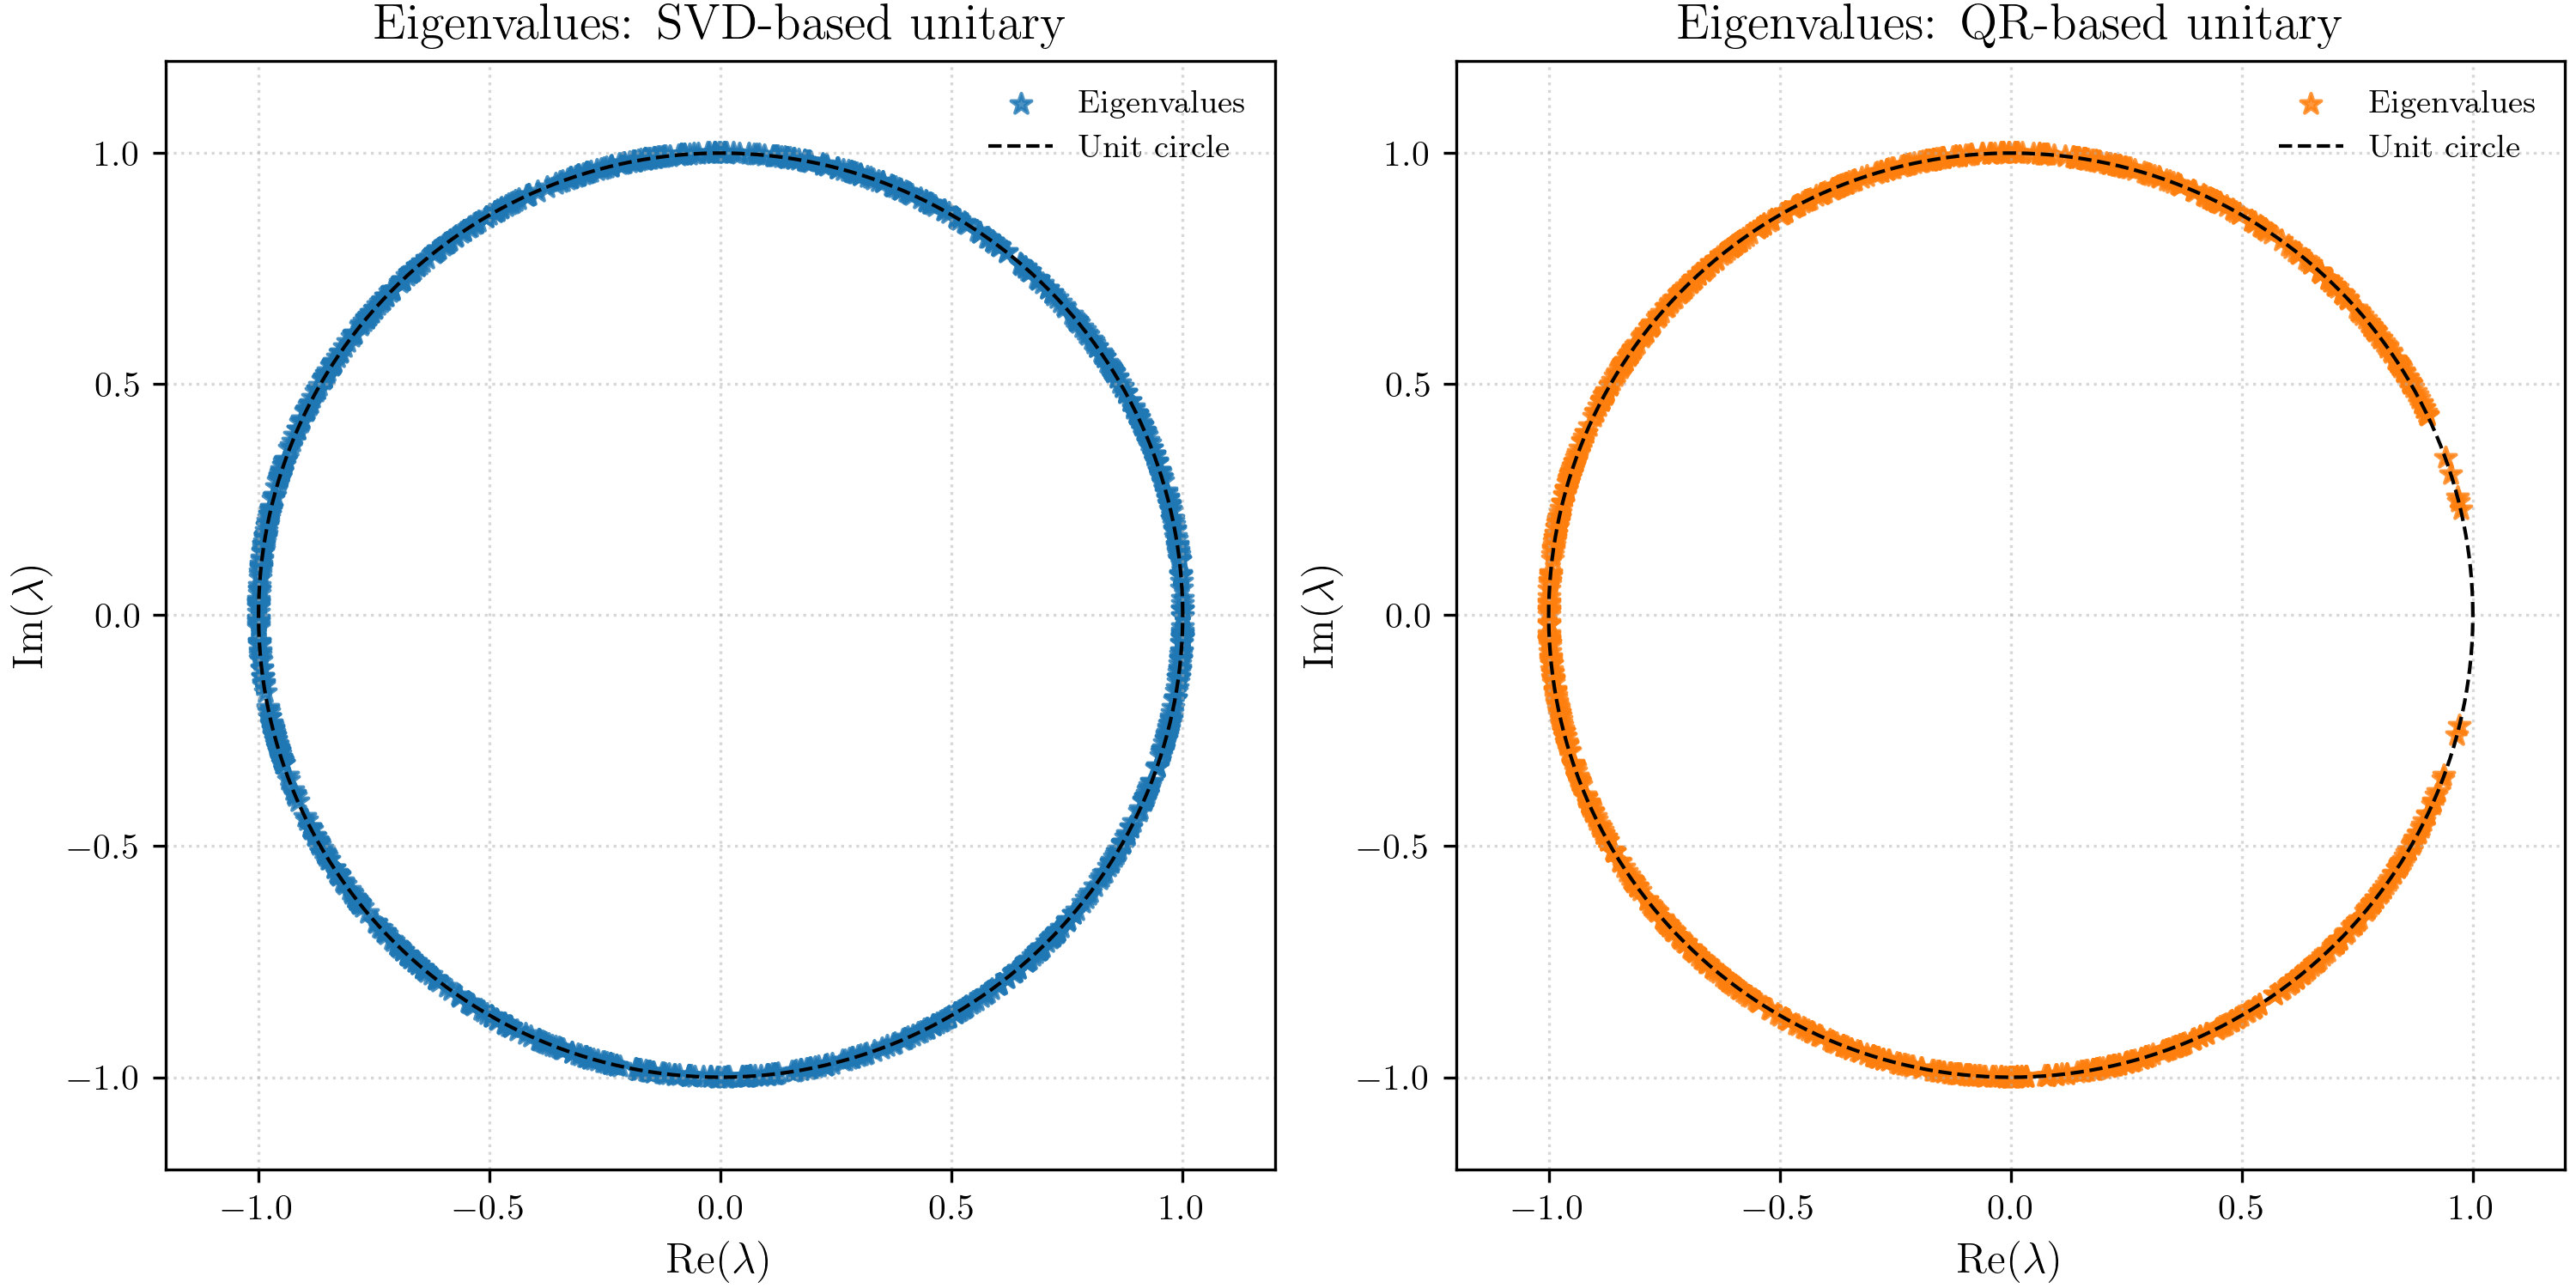
\includegraphics[width=1\textwidth]{Graphics/eigenvalue_comparison.png}
    \caption{Eigenvalue distributions of random unitary matrices generated via SVD and QR.}
    \label{fig:eigenvalue-comparison}
\end{figure}

\section{Spectral Density}

To get to the notion of the spectral density,
we will first need some more basic definitions to build on.
The reader is assumed to be familiar with the concepts of distributions.
Let us also recap that for $\Omega \subset \C^n$ open and non-empty,
a \emph{test function} is a smooth function with compact support defined on $\Omega$.
The space of all test functions on $\Omega$ is usually denoted by $\mathcal{E}$.

We will now look at an important case of a distribution

\begin{definition}[Dirac delta distribution]
    Let $\mathcal{E} = \Cinfty(\Omega)$ with $0 \in \Omega \subset \R^n$.
    Then
    $$\delta: \mathcal{E} \to \R, \quad f \mapsto f(0) \quad \text{with} \quad \delta(f) = \langle \delta, f \rangle = f(0)$$
\end{definition}

this distribution is often mistakenly referred to as a function,
although it is not a function in the classical sense.\\
The Dirac delta is characterized by the following property:

\[
\int\limits_{-\infty}^{\infty} f(x) \delta(x-a) \dx = \int\limits_{-\infty}^{\infty} f(x) \delta(a-x) \dx = f(a) \implies \int\limits_{-\infty}^{\infty} \delta(x-a) \dx = 1.
\]

This means that the Dirac delta distribution is zero everywhere except at the point $a$,
where it is infinitely high, such that the integral over it equals $1$.
We now have all the tools we need to define the central concept of this thesis:

\begin{definition}[Spectral density]
    Let $H$ be hermitian and sparse.
    For $x \in \R$, the \emph{spectral density} is then defined as
    \[
    \phi(x) = \frac{1}{n} \sum_{j=1}^{n} \delta(x - \lambda_j)
    \]
    where $\delta$ is the Dirac delta distribution
    and $\lambda_j$ are the eigenvalues of $H$ in non-descending order.
\end{definition}

The number of eigenvalues in an interval $[a, b]$ can then be counted in the following manner:

\begin{equation} \label{eq:nu_a_b}
    \nu_{[a, b]} = \int\limits_a^b \sum_j \delta(t - \lambda_j) \dt \equiv \int\limits_a^b n \phi(t) \dt
\end{equation}

Random matrix theory tells us that the eigenvalues of random unitary matrices are distributed uniformly on the unit circle.
Thus, we would expect the spectral density to be uniformly distributed on the unit circle as well.
This is important as we think of the choice of random unitary matrices.

If we generate a random complex square matrix $A$,
there are multiple ways to obtain a unitary matrix $U$.
We will now compare the svd with the qr decomposition.

Before we can proceed to the motice of this thesis, we will need to define the following space:

\begin{definition}[Schwartz space over $\R$] \label{def:Schwartz space}
    The \emph{Schwartz space} over $\R$ consists of all smooth functions $f$ that decay rapidly to zero as $|x|$ approaches infinity \cite{richtmyer}.
    Formally,
    \[
    \SR := \left\{f \in \Cinfty(\R) \mid \forall p, k \in \N_0: \sup_{x \in \R} \left| x^p f^{(k)}(x) \right| < \infty \right\}
    \]
\end{definition}